\section{Method}
\label{sec:method}

This thesis aims to produce a working implementation of an application with visual as well as natural-language input, using \gls{ttr}.
Such an application largely resembles those put forward in \cite{lspc} and \cite{ttrspat}, but there are some differences.
This application will feature:

\begin{enumerate}
\item Sensory input in the form of 2D images
\item Utilizing an external object recognition system
\item Detection of geometric spatial relations
\item Basic natural language understanding
\end{enumerate}

While operational functionality and the overall procedural code is written in Python, the core model is written in \gls{ttr} (realized as Python code using PyTTR).
As such, \gls{ttr} serves as a formal specification language.
The additional layer provides formal transparency and type robustness.

This section will describe some reasoning around the decisions taken, regarding the design of the \gls{ttr} model as well as its implementation.



\subsection{Object detection with YOLO}

You only look once (YOLO) \citep{RedmonYouOnlyLook2015} is a neural network model for image recognition.
It is trained using a loss function which takes detection as well as classification into account.
In other words, it simultaneously predicts bounding boxes and classifies the contained objects.
Unlike \cite{HeMaskRCNN2017} and others, it does not contain any recurrent layers.
The joint, recurrence-free model makes for a rather small network size, which in turn means a favorable evaluation speed.
However, compared to state of the art, it lags behind in accuracy.

[training]

\begin{figure}[h]
\label{fig:dogbike_annotated}
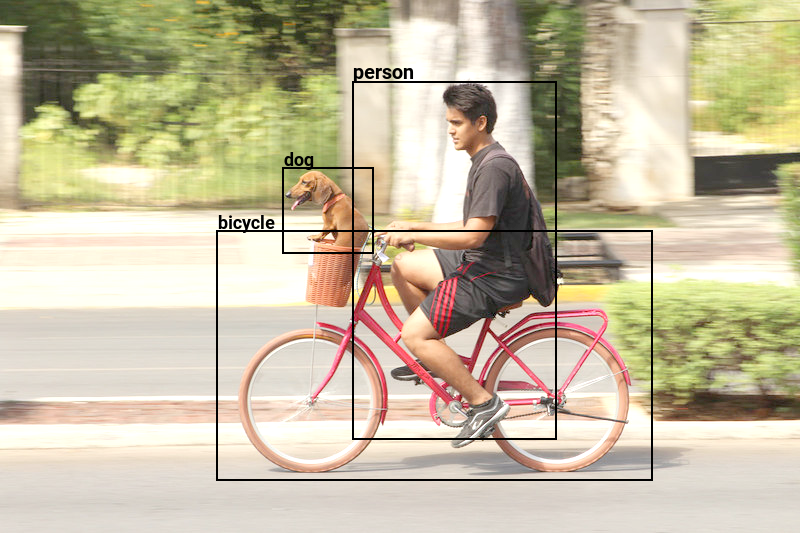
\includegraphics[width=\textwidth]{dogbike_annotated}
\centering
\caption{Visualization of the labels and bounding boxes emitted by YOLO when given an image depicting a cyclist with a dog.}
\end{figure}

YOLO is written in C, using the Darknet neural network library \citep{darknet13}.
It can be used in Python with the TensorFlow machine learning library and the Darkflow library which translates a Darknet model to TensorFlow.

When invoked from Python, the return value is a collection of dict objects, each containing a label, coordinates and a confidence score, as exemplified in \autoref{lst:yolo_out}.
Results with confidence over a certain threshold are cast into \gls{ttr} records as described in \autoref{ssec:python}.

\begin{lstlisting}[label=lst:yolo_out, caption=Example output of YOLO invocation]
[
	{
		'topleft': {'x': 354, 'y': 86},
		'bottomright': {'x': 551, 'y': 437},
		'label': 'person',
		'confidence': 0.80116189
	},
	{
		'topleft': {'x': 224, 'y': 234},
		'bottomright': {'x': 646, 'y': 476},
		'label': 'bicycle',
		'confidence': 0.85828924
	},
	...
]
\end{lstlisting}



\subsection{Objects and perception}

Our model of the perception of objects is largely based on \cite{lspc}.
In short, a \textit{perceptual object} (a record) is used to generate an \textit{individuated object} (a record type) as well as a witness for the situation described by the individuated object. [rewrite, some more detail?]
More on this in \autoref{ssec:ttrmodel}.

In \cite{lspc}, however, the input space is a 3D point space rather than 2D images.
This necessitates different types for the perceptual input and the locations of perceived objects.
In the point space case, the $PointMap$ set type is used for the full ``world'', and any part of the world is simply a subset of it, so it is also a $PointMap$.
In our case, $Image$ is used for the full image but we use $Segment$ to refer to parts of it.

[propositions as types, true if there is an object of the type, situation semantics? \cite{BarwiseSituationsAttitudes1981}]
A record of a situation type then serves as a witness for the situation.



\subsection{Spatial relations}
% Classification algorithm non-TTR. Simplistic, compare to sophisitcated alternatives.

Spatial relation classification is mostly based on \cite{ttrspat}, but more simplistic.

\cite{ttrspat} includes two important aspects that are not covered here.
First, it assumes a 3D point space as visual input, in contrast to the 2D image considered here.
Spatial relations in 3D crucially involves adapting the reference frame according to the viewpoint, while those are trivially fixed in the 2D case.
Second, it accounts for the functional aspect of spatial relationship, as detailed by \cite{CoventryClassificationExtrageometricInfluences2004}.

A spatial classifier $\kappa$ takes two locations and returns a boolean result.
We have implemented spatial classifiers as Python functions.
For the purpose of this thesis, no sophisticated spatial classification has been considered.
Instead, a naive comparison between centers of bounding boxes was implemented.
This was done for the four relations ``left'', ``right'', ``above'' and ``below''.



\subsection{Language and \gls{vqa}}
\label{ssec:languagevqa}

We focus on validating declarative utterances, which corresponds to answering a yes/no questions.
Other question types are not considered.

The utterance is parsed.
The resulting type is compared to that of the scene.
This is multimodality.

The existing research on \gls{ttr}-based approaches to textual or phonetic parsing, overviewed in \autoref{ssec:ttnlp}, would surely cover the kind of utterances considered here.
However, there is currently no implementation available and ready to use, and parsing is not within the main focus of this thesis.
Therefore, the natural-language parsing implemented for this thesis is instead a simplistic one.
It uses feature structure context-free grammar (FCFG) tools available in NLTK \cite{BirdNaturalLanguageProcessing2009} to parse text into \gls{fol} expressions.
With a custom function {\tt fopc\_to\_pyttr}, the \gls{fol} expressions are transformed to a TTR record type.

A dog is to the left of a car
\begin{equation}\left[\begin{array}{rcl}
\text{x} &:& Ind\\
\text{y} &:& Ind\\
\text{c}_\text{dog} &:& \text{dog}(x)\\
\text{c}_\text{car} &:& \text{car}(y)\\
\text{c}_\text{left} &:& \text{left}(x, y)\\
\end{array}\right]\end{equation}

The fact that the natural-language utterance is given a representation in the same formal framework as the image allows comparing them to each other.
Essentially, we would like to check if the situation observed is a subtype of the situation described by the question: whether $Q \sqsupseteq A$.
However, we need not to impose the requirement that field labels should match, which is a necessity for the subtype relation to hold.
Thus, the condition is reformulated to allow relabeling \citep[pp. 133–135]{CooperTypetheorylanguage2016}:

If $Q$ is the type of a polar question utterance and $A$ is the type of the scene, the answer is YES if there is a relabeling $\eta$ such that $A \sqsubseteq Q_\eta$, and otherwise it is NO.

[classification before/after question]



\subsection{Evaluation}

The system is tested on a few sentences for a few images.
...
